\documentclass{beamer}
\usepackage[english,russian]{babel}
\usepackage[utf8]{inputenc}
\usetheme[numbers]{Warsaw}

\begin{document}

\institute{МГУ имени М.В. Ломоносова, Москва, Россия}
\title{Отчёт по второму заданию}  
\author{Пахомова, Пантелеева, Кулик, 411 группа}
\date{ 2016\\Москва} 
\thispagestyle{empty}
\frame{\titlepage} 

\begin{frame}{Описание задания}

{\small
Целью второго задания было проведение разведывательного анализа данных для того, чтобы определить, с каким из поставщиков стали следует заключить договор, основываясь на имеющихся данных по производству оружия и количеству единиц сломанного оружия за каждый месяц каждым из кузнецов двух анализируемых компаний. }

\end{frame}

\begin{frame}{Описание решения}

{\footnotesize
С помощью диаграммы размаха («Ящик с усами») исследуем эффективность производства каждой из компаний.

По оси абсцисс указаны рассматриваемые компании, по оси ординат значения вектора количества целых мечей, произведённых компанией, посчитанных следующим образом:

Из значения количества произведённых мечей в партии вычитается сумма количества сломанных мечей от рассматриваемой партии на данный момент времени, все значения берутся суммарно по всем кузнецам компании.
Т.е. если в первый месяц было произведено Х мечей всеми кузнецами компании, и за 6 месяцев сломалось Y мечей от произведенного X, то первым элементом вектора будет значение (X - Y), и т.д.

Таким образом на диаграмме размаха видим медиану значений (выделенная жирной линией), максимальное значение в выборке (верхней чертой) и минимальное (нижней чертой). }

\end{frame}


\begin{frame}{Описание решения}	
	\begin{figure}[h]
		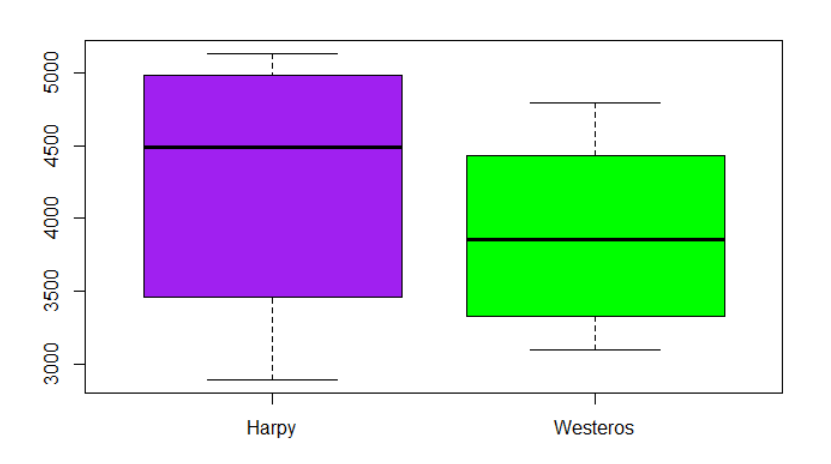
\includegraphics[width=100mm]{Graph}
		\caption{"Диаграммы размаха"}
		\label{Graph}
	\end{figure}
	
\end{frame}

\begin{frame}{Анализ результатов}

{\small
Далее анализируем полученный после выполнения программы график.

1) Разброс максимальных и минимальных значений количества целых мечей больше у компании Harpy & Co, нежели чем у компании Westeros Inc.. Это означает, что у второй компании качество партий не так сильно отличается друг от друга, что показывает стабильность производства и является плюсом.

2) Медиана количества целых мечей у компании Harpy & Co больше, чем у компании Westeros Inc.. Это означает, что в среднем качество мечей первой компании всё же выше, чем у второй.}

\end{frame}

\begin{frame}{Анализ результатов}

{\small
Далее по полученным анализам делаем вывод, с какой компанией следует сотрудничать.
Поскольку контракт будет заключаться на долговременный период (т.е. 11 месяцев), значение медианы имеет больший вес, чем разброс максимальных и минимальных значений. Следовательно, делаем вывод, основываясь на результатах анализа медианы.

Таким образом, наиболее выгодно будет заключить контракт с компанией Harpy & Co.}

\end{frame}

\begin{frame}{Задание выполняли}
	\begin{itemize}
		{\small
		\item Пахомова Маргарита, студентка 411 группы. Написание программы
		\item Пантелеева Анастасия, студентка 411 группы. Написание Rnotebook и презентации
		\item Кулик Артем, студент 411 группы. Написание программы}
	\end{itemize}	

\end{frame}

\end{document}
